\documentclass[xcolor=svgnames,handout]{beamer}

\usepackage[utf8]    {inputenc}
\usepackage[T1]      {fontenc}
\usepackage[english, russian] {babel}

\usepackage{amsmath,amsfonts,graphicx}
\usepackage{beamerleanprogress}
\usepackage{tikz}
\usepackage[outline]{contour}
\usepackage{hyperref}

\title
  [Music Genre Classification\hspace{2em}]
  { \color{black}\contour{SkyBlue}{Multilingual I-Vector based Statistical} \contour{SkyBlue}{Modeling for Music Genre Classification}\vspace{1.5cm} }

\author
  []
  {Трубицын Юрий \\ Пиджакова Анна \\ Ходырева Виктория}

\date
  {\textbf{Июнь, 2018}}

\institute
  {\textbf{МГУ им. Ломоносова}}


\begin{document}



    
            
{
  \begin{frame}
  %current page.center
    \begin{tikzpicture}[remember picture, overlay]
    \shade[top color=grey!23,bottom color=grey!23,middle color=white]
  ([shift={(0.25cm,-0.25cm)}]current page.north west)
     rectangle
  ([shift={(-0.25cm,0.25cm)}]current page.south east);
    \node[scope fading=west, opacity=0.5,inner sep=0pt] at (current page.center) %(5.7,0.5)
    {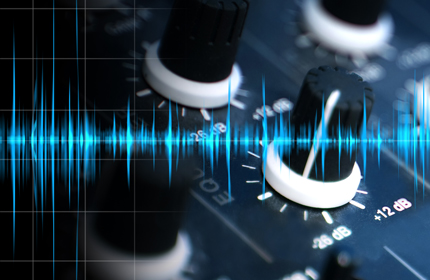
\includegraphics[width=\paperwidth,height=\paperheight]{pic1.jpg}};

  \end{tikzpicture}

   \vspace{0.5cm}
    \titlepage
  \end{frame}
}

\section
  {Постановка задачи}
\begin{frame}
  {Постановка задачи}

%   Things in a Bulleted List\pause

%   \begin{itemize}
%   \item Bullets that\pause
%   \item Come up\pause
%   \item One by one
%   \end{itemize}

  \begin{block}{Задача}
    Автоматическое распознавание жанра музыкального \\произведения 
  \end{block}
  \begin{minipage}{0.45\textwidth}
  \begin{flushleft}
  Мотивация:
  \begin{itemize}
      \item У музыкальных жанров нет четких границ и характеристик
      \item Ручная разметка стоит дорого
      \item Широкий спектр применений: поиск, сортировка музыки
      \item Pandora, Spotify
  \end{itemize}
  \end{flushleft}
  \end{minipage}
  \begin{minipage}{0.47\textwidth}
  \begin{flushright}
	\begin{figure}[H]
        \begin{minipage}[h]{0.3\linewidth}
        \center{
\includegraphics[width=1\linewidth]{pandora}\\}
        \end{minipage}
        \hfill
        \begin{minipage}[h]{0.67\linewidth}
        \center{
\includegraphics[width=1\linewidth]{spotify-1}\\}
        \end{minipage}
        \vfill
        \vfill
        \begin{minipage}[h]{0.99\linewidth}
        \center{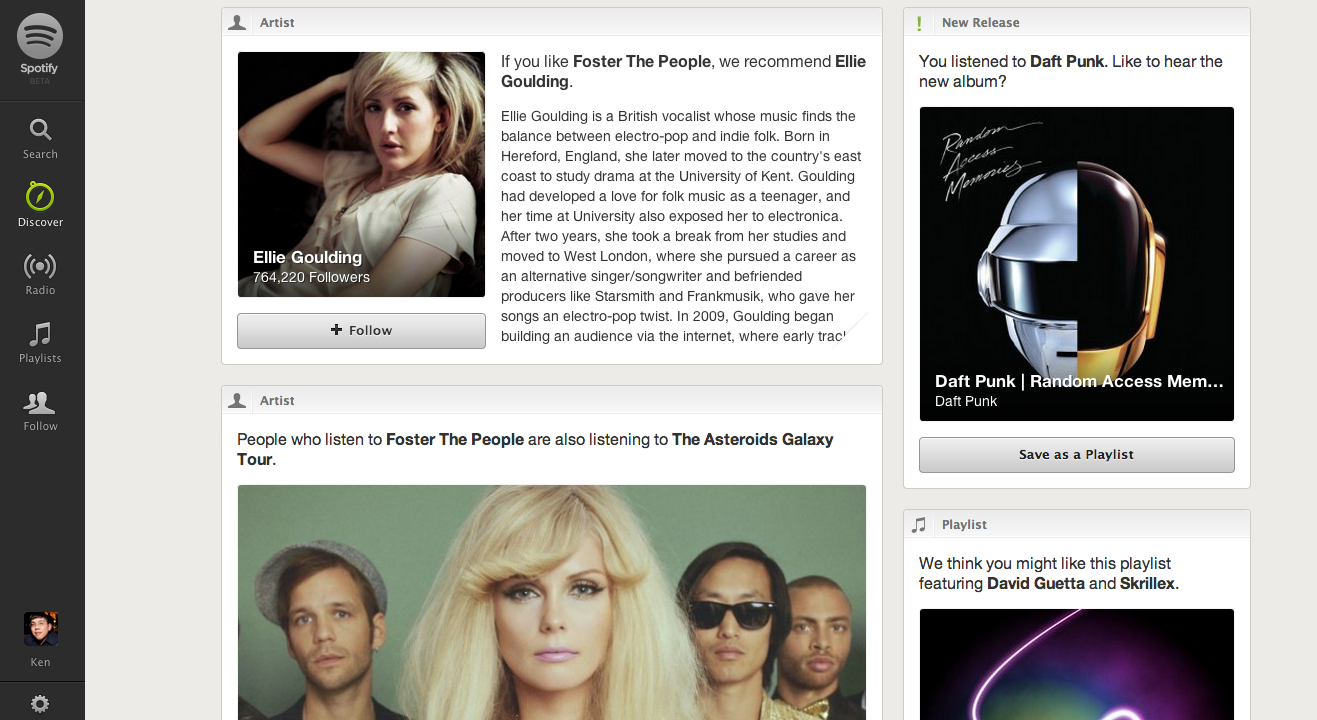
\includegraphics[width=1\linewidth]{spotify}}
        \end{minipage}
    \end{figure}

  \end{flushright}
\end{minipage}
  
\end{frame}

  
\begin{frame}
  {Данные}
  Использовался датасет Marsyas (Music Analysis, Retrieval, and Synthesis for Audio Signal)
    
  \begin{figure}[t]
    \centering
    
\includegraphics[width = 0.95\linewidth]{header}
  \end{figure}
  
  \textbf{Описание датасета}
  \begin{itemize}
      \item состоит из 1000 аудио треков по 30 секунд каждый;
      \item все файлы разделены на 10 жанров;
      \item каждому жанру соответствует 100 треков;
  \end{itemize}


\end{frame}


\section
  {Обзор литературы}
  
\begin{frame}{Обзор литературы}
%   \textbf{M. Haggblade, Y. Hong: "Music Genre Classification"}
  \begin{block}{M. Haggblade, Y. Hong: Music Genre Classification}
  \begin{itemize}
      \item Базовые признаки -- MFCC-коэффициенты
      \item \texttt{Идея}: Применить k-means, k-Nearest Neighbors (k-NN) и много-классовую SVM для полученных признаков используя в качестве расстояния KL-дивергенцию. А так же обучить нейронную сеть.
  \end{itemize}
  \end{block}
    \begin{figure}[t]
    \centering
    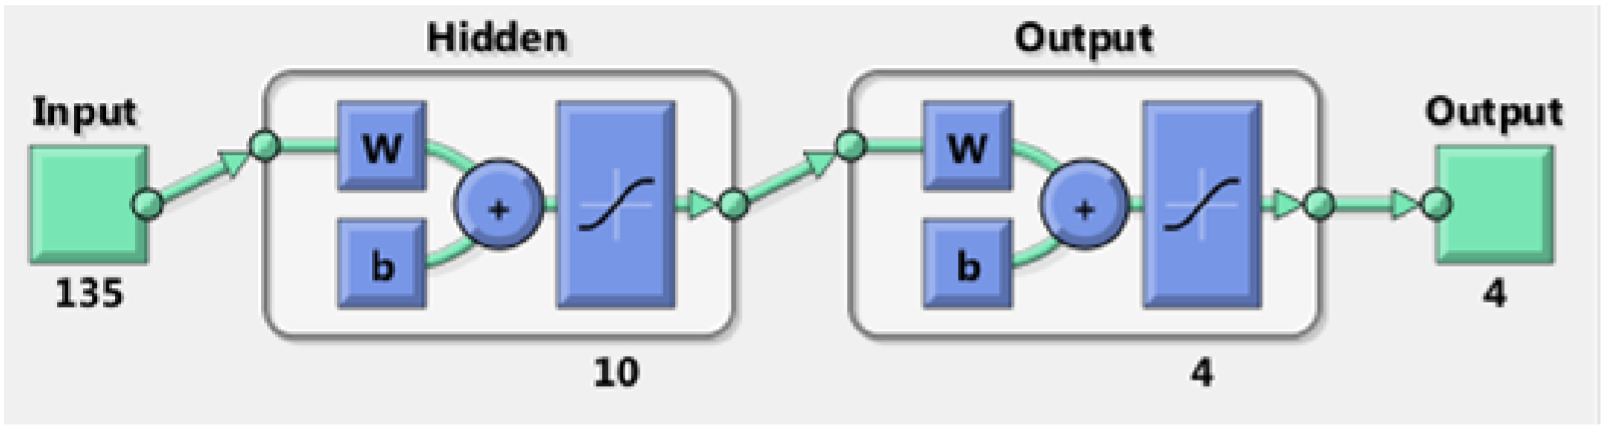
\includegraphics[width = 0.95\linewidth]{nn-structure}
  \end{figure}
\end{frame}


\begin{frame}
%   \textbf{G. Tzanetakis: "Musical Genre Classification of Audio Signals"}
  \begin{block}{G. Tzanetakis: Musical Genre Classification of Audio Signals}
  \begin{itemize}
      \item Базовые признаки -- MFCC-коэффициенты
      \item Модифицированные признаки:
      \begin{itemize}
          \item текстура тембра;
          \item спектральный спад частотной характеристики;
          \item спектральный поток;
          \item анализ и текстура фрейма и т.д.;
      \end{itemize}
      \item \texttt{Идея}: для инициализации GMM класификатора с диагональной матрицей ковариации используется k-means, стартующий из случайных точек.
  \end{itemize}
  \end{block}
  \begin{block}{Joakim Anden: Deep Scattering Spectrum}
%   \textbf{Joakim Anden: "Deep Scattering Spectrum"}
  \begin{itemize}
      \item Интересное: для улучшения качества предсказания вместо MFCC-коэффициентов используется scatter MFCC.
  \end{itemize}
  \end{block}
\end{frame}  

\section
  {i-vector}


\begin{frame}
  {Построение высокоуровневых признаков}
\begin{figure}[t]
    \centering
    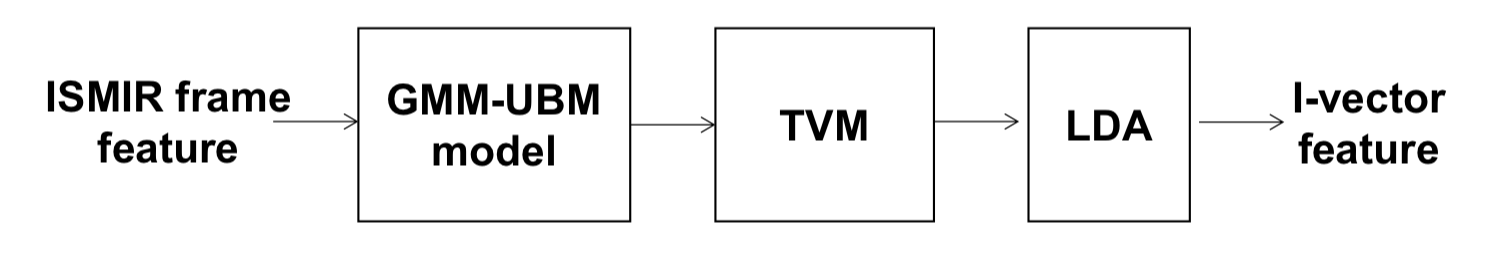
\includegraphics[width = 0.95\linewidth]{pipe.png}
  \end{figure}
  
    \begin{itemize}
    \item Выделение низкоуровневых признаков: MFCC
    \item Построение универсальной GMM-UBM модели
    \item Вычисление супервектора GMM, используя статистику BW 
    \item Снижение размерности с использованием TVM для получение i-vector (unsupervised)
    \item Снижение размерности i-vector с помощью LDA (supervised)
    \end{itemize}

\end{frame}

  
\begin{frame}
  {GMM-UBM + TVM}

    \begin{itemize}
    \item $i=[1,\ldots,  C]$ - компоненты смеси гауссиан,\\ $t=[1,\ldots,  T]$ - фреймы аудиозаписи, \\
    $x_t$ - MFCC признаки фрейма $t$
    \item GMM: $b_i(x_t)$ - апостериорная вероятность фрейма $x_t$ принадлежности $i$-той компоненте 
    \item $E_i^0 = \sum\limits_t{b_i(x_t)}$\\
          $E_i^1 = \sum\limits_t{b_i(x_t)x_t}$ \\
          $E_i^2 = \sum\limits_t{b_i(x_t)x_tx_t^T}$
    \item $m_i = \frac{E_i^1}{E_i^0}$ \\
          $M = [m_1, m_2, \ldots, m_T]$ - супервектор GMM
    \item $M = m_0+Tw$, $m_0$ - медианы компонент, $T$-матрица TVM, \\$w$ - i-vector
    \end{itemize}

\end{frame}

  
\begin{frame}
  {Процесс извлечения i-vector}

  \begin{figure}[t]
    \centering
    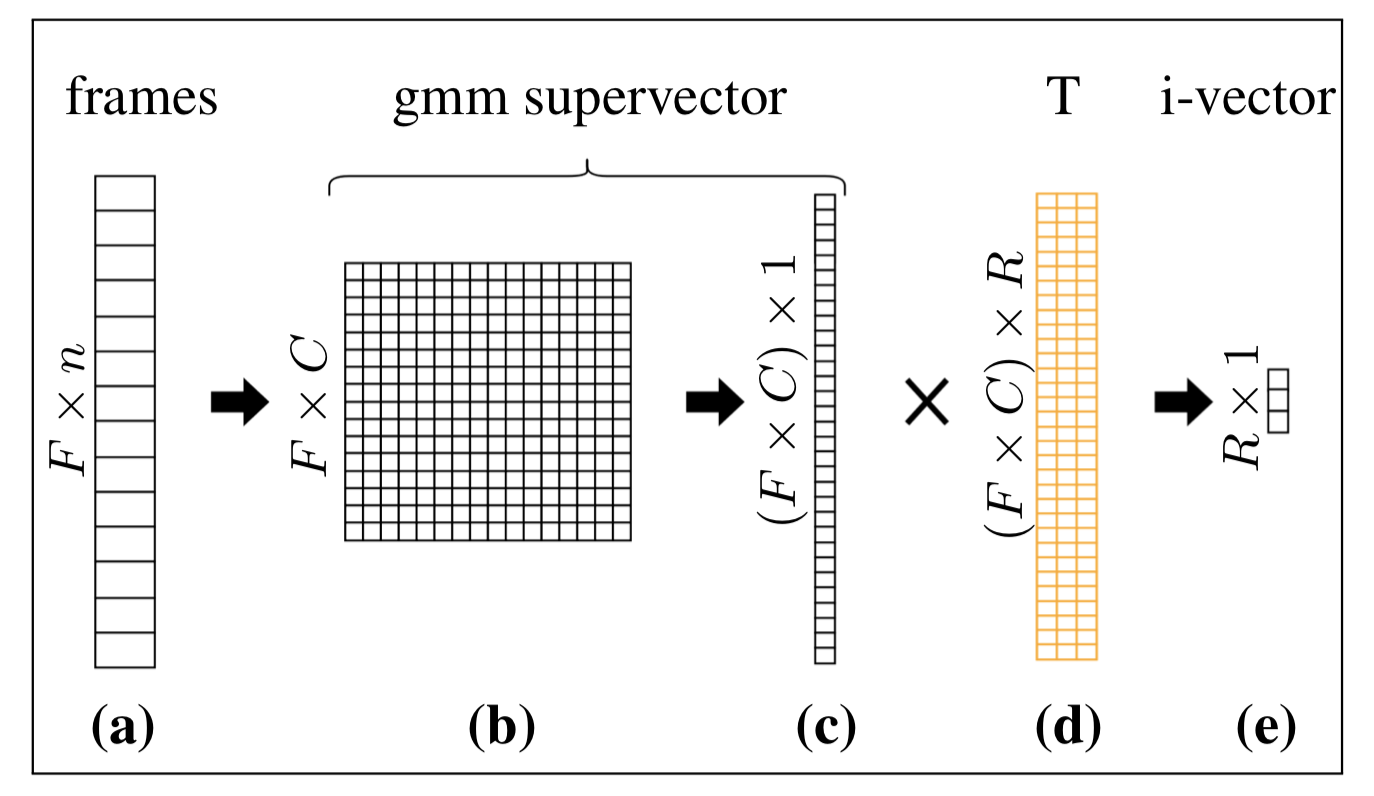
\includegraphics[width = 0.95\linewidth]{ivector.png}
  \end{figure}
 
 
\end{frame}

\section
  {Результаты}
  
  
  
\begin{frame}{Baseline 1}
  DNN (39-128-3)
  \begin{figure}[t]
    \centering
    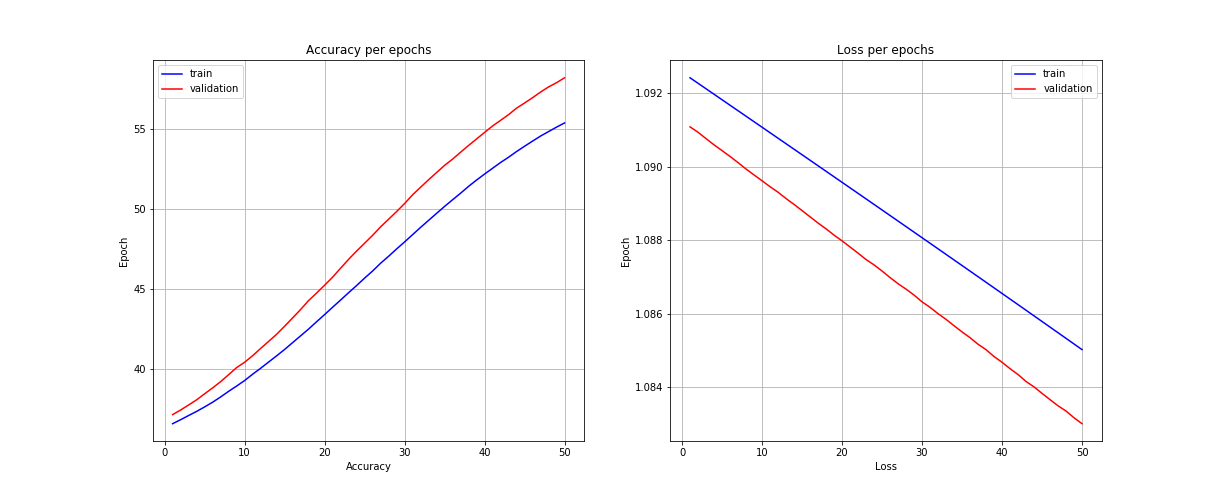
\includegraphics[width = 1\linewidth]{results_dnn.png}
  \end{figure}
  Accuracy = 0.62
 \end{frame}
 
 
 \begin{frame}{Baseline 2}
  DNN (39-128--512-128-9)
  \begin{figure}[t]
    \centering
    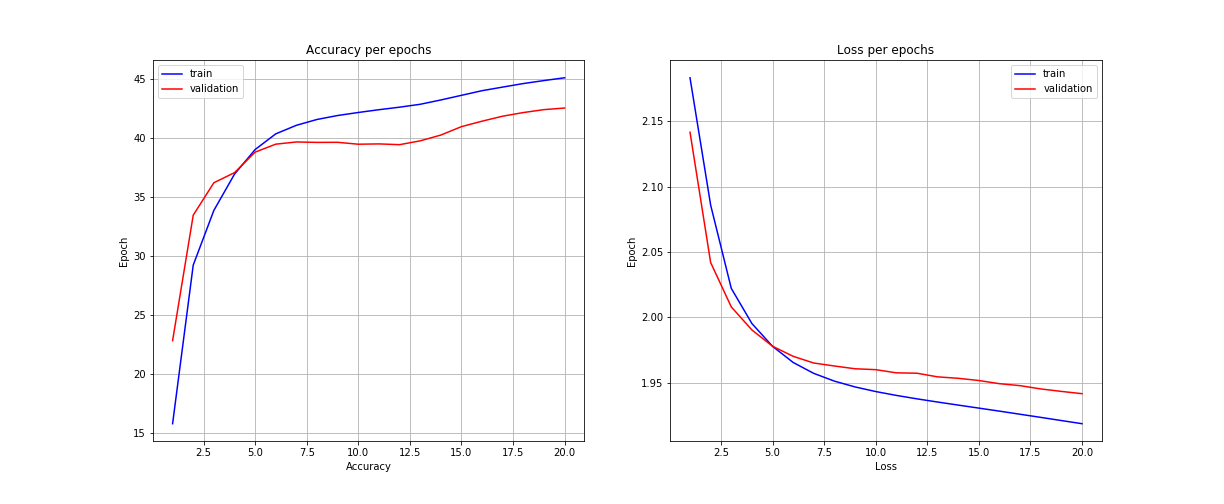
\includegraphics[width = 1\linewidth]{results_dnn_512.png}
  \end{figure}
  Accuracy = 0.46
 \end{frame}

 \begin{frame}{I-vector}
  \begin{itemize}
      \item \textbf{GMM-UBM200 + TVM400}: accuracy = 0.83
      \item \textbf{GMM-UBM200 + TVM800}: accuracy = 0.96
      \item \textbf{GMM-UBM200 + TVM400 + lda2}: accuracy = 0.66
  \end{itemize}
 \end{frame}


\begin{frame}
  {Вклад участников}

  \begin{enumerate}
      \item Трубицын Юрий
      \begin{itemize}
      \item Предобработка данных
      \item Работа над бейзлайном
      \item Администрирование GitHub
      \end{itemize}
      \item Пиджакова Анна
      \begin{itemize}
      \item Обзор литературы
      \item Оформление презентации
      \item Применение методов GMM, TVM
      \item Обучение модели SVM
      \end{itemize}
      \item Ходырева Виктория
      \begin{itemize}
      \item Оформление презентации
      \item Обзор библиотек для получения i-vector
      \item Применение LDA для снижения размерности
      \item Оценка качества SVM
      \end{itemize}
  \end{enumerate}
 
 
\end{frame}

\begin{frame}
  {Список литературы}

  \begin{itemize}
  \item \href{https://www.isca-speech.org/archive/Interspeech_2017/pdfs/0074.PDF}{J. Dai, W. Xue, W. Liu: Multilingual I-Vector based Statistical Modeling for Music Genre Classification}
  \item \href{http://ismir2015.uma.es/articles/128\_Paper.pdf}{H. Eghbal-zadeh, B. Lehner, M. Schedl, G. Widmer: I-VECTORS FOR TIMBRE-BASED MUSIC SIMILARITY AND MUSIC ARTIST CLASSIFICATION}
  \item \href{http://cs229.stanford.edu/proj2011/HaggbladeHongKao-MusicGenreClassification.pdf}{M. Haggblade, Y. Hong: Music Genre Classification}
  \item \href{https://www.researchgate.net/publication/220656193_Musical_Genre_Classification_of_Audio_Signals}{G. Tzanetakis: Musical Genre Classification of AudioSignals}
  \item \href{https://arxiv.org/abs/1304.6763}{Joakim Anden: Deep Scattering Spectrum}
  \end{itemize}
  
\end{frame}


\begin{frame}
  
  
  \begin{tikzpicture}[remember picture, overlay]
    \node[scope fading=west, opacity=0.5,inner sep=0pt] at (5.5,-3) %(5.7,0.5)
    {
\includegraphics[width=\paperwidth,height=100]{sound.png}};
  \end{tikzpicture}
  \vspace{-1.5cm}
  \center{\color{black}\contour{SkyBlue}{\large{Спасибо за внимание!}} \\
  \vspace{0.5cm}
  \color{black}\contour{SkyBlue}{Самое время задать вопросы :)} }
  

  
\end{frame}

\end{document}

